\begin{appendix}
\chapter{Anexo: Figuras del �rbol de Objetivos y El �rbol de Problemas}\label{AnexoA}
\begin{figure}[!ht]
\centering
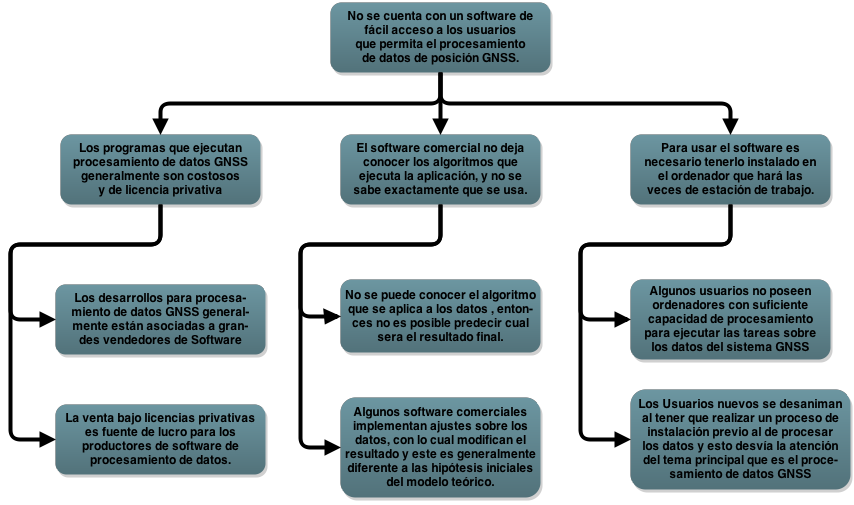
\includegraphics[width=16cm]{Kap3/Fig_Kap3/ArboldeProblemas.png} %height=8cm,
\caption[�rbol de Problemas]{Gr�fica del �rbol de Problemas}
\label{fig:ArProblem}
\end{figure}

\begin{figure}[!ht]
\centering
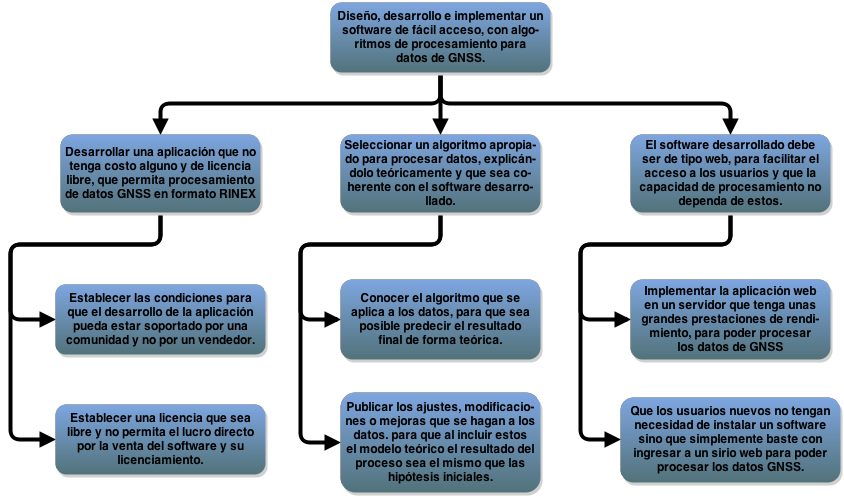
\includegraphics[width=16cm]{Kap3/Fig_Kap3/ArboldeObjetivos.png} %height=8cm,
\caption[�rbol de Objetivos]{Gr�fica del �rbol de Objetivos}
\label{fig:ArObjetivos}
\end{figure}

%\chapter{Anexo: Nombrar el anexo B de acuerdo con su contenido}
%A final del documento es opcional incluir \'{\i}ndices o glosarios. \'{E}stos son listas detalladas y especializadas de los t\'{e}rminos, nombres, autores, temas, etc., que aparecen en el mismo. Sirven para facilitar su localizaci\'{o}n en el texto. Los \'{\i}ndices pueden ser alfab\'{e}ticos, cronol\'{o}gicos, num\'{e}ricos, anal\'{\i}ticos, entre otros. Luego de cada palabra, t\'{e}rmino, etc., se pone coma y el n\'{u}mero de la p\'{a}gina donde aparece esta informaci\'{o}n.\\
%
%\chapter{Anexo: Nombrar el anexo C de acuerdo con su contenido}
%MANEJO DE LA BIBLIOGRAF\'{I}A: la bibliograf\'{\i}a es la relaci\'{o}n de las fuentes documentales consultadas por el investigador para sustentar sus trabajos. Su inclusi\'{o}n es obligatoria en todo trabajo de investigaci\'{o}n. Cada referencia bibliogr\'{a}fica se inicia contra el margen izquierdo.\\
%
%La NTC 5613 establece los requisitos para la presentaci\'{o}n de referencias bibliogr\'{a}ficas citas y notas de pie de p\'{a}gina. Sin embargo, se tiene la libertad de usar cualquier norma bibliogr\'{a}fica de acuerdo con lo acostumbrado por cada disciplina del conocimiento. En esta medida es necesario que la norma seleccionada se aplique con rigurosidad.\\
%
%Es necesario tener en cuenta que la norma ISO 690:1987 (en Espa\~{n}a, UNE 50-104-94) es el marco internacional que da las pautas m\'{\i}nimas para las citas bibliogr\'{a}ficas de documentos impresos y publicados. A continuaci\'{o}n se lista algunas instituciones que brindan par\'{a}metros para el manejo de las referencias bibliogr\'{a}ficas:\\
%
%\begin{center}
%\centering%
%\begin{tabular}{|p {7.5 cm}|p {7.5 cm}|}\hline
%\arr{Instituci\'{o}n}&Disciplina de aplicaci\'{o}n\\\hline%
%Modern Language Association (MLA)&Literatura, artes y humanidades\\\hline%
%American Psychological Association (APA)&Ambito de la salud (psicolog\'{\i}a, medicina) y en general en todas las ciencias sociales\\\hline
%Universidad de Chicago/Turabian &Periodismo, historia y humanidades.\\\hline
%AMA (Asociaci\'{o}n M\'{e}dica de los Estados Unidos)&Ambito de la salud (psicolog\'{\i}a, medicina)\\\hline
%Vancouver &Todas las disciplinas\\\hline
%Council of Science Editors (CSE)&En la actualidad abarca diversas ciencias\\\hline
%National Library of Medicine (NLM) (Biblioteca Nacional de Medicina)&En el \'{a}mbito m\'{e}dico y, por extensi\'{o}n, en ciencias.\\\hline
%Harvard System of Referencing Guide &Todas las disciplinas\\\hline
%JabRef y KBibTeX &Todas las disciplinas\\\hline
%\end{tabular}
%\end{center}
%
%Para incluir las referencias dentro del texto y realizar lista de la bibliograf\'{\i}a en la respectiva secci\'{o}n, puede utilizar las herramientas que Latex suministra o, revisar el instructivo desarrollado por el Sistema de Bibliotecas de la Universidad Nacional de Colombia\footnote{Ver: www.sinab.unal.edu.co}, disponible en la secci\'{o}n "Servicios", opci\'{o}n "Tr\'{a}mites" y enlace "Entrega de tesis".

\end{appendix}
